% !TeX document-id = {b09344d7-b33e-4195-b30b-ef42e3d16afe}
% !TeX TXS-program:compile = txs:///pdflatex | txs:///makeglossaries
% | txs:///pdflatex | txs:///pdflatex
%%%%%%%%%%%%%%%%%%%%%%%%%%%%%%%%%%%%%%%%%
% Simple Sectioned Essay Template
% LaTeX Template
%
% This template has been downloaded from:
% http://www.latextemplates.com
%
% Note:
% The \lipsum[#] commands throughout this template generate dummy text
% to fill the template out. These commands should all be removed when
% writing essay content.
%
%%%%%%%%%%%%%%%%%%%%%%%%%%%%%%%%%%%%%%%%%

%----------------------------------------------------------------------------------------
%  PACKAGES AND OTHER DOCUMENT CONFIGURATIONS
%----------------------------------------------------------------------------------------

\documentclass[hidelinks, 12pt]{article} % Default font size is 12pt,
% it can be changed here

\usepackage[table,xcdraw]{xcolor} % colored table package

\usepackage{geometry} % Required to change the page size to A4
%\geometry{a4paper} % Set the page size to be A4 as opposed to the
% default US Letter

\usepackage{graphicx} % Required for including pictures
\usepackage{adjustbox}
\usepackage{float} % Allows putting an [H] in \begin{figure} to
% specify the exact location of the figure
\usepackage{wrapfig} % Allows in-line images such as the example fish picture
\usepackage{setspace} % To control linespacing
\usepackage{enumerate} % For enumerating lists
\usepackage{enumitem} % more enumerating stuff
\usepackage{multicol} % for multicoumn formating
\usepackage{multirow} % for multicoumn formating
\usepackage{adjustbox}
\usepackage{changepage}
\usepackage{fancyhdr}
\usepackage[usenames,dvipsnames]{xcolor} %To change text colors,
% color options located at: http://en.wikibooks.org/wiki/LaTeX/Colors
% \usepackage[font={footnotesize}]{caption}
\usepackage[labelfont=bf]{caption}
\usepackage{longtable}
\usepackage{tabularx}
\usepackage{arydshln}
\usepackage{titlesec} % To control section colors
\usepackage{color}
\usepackage{hyperref} % for web links
\usepackage{subcaption}% Specifies the directory where pictures are stored
\usepackage[toc, acronym, nopostdot, nonumberlist, nomain]{glossaries}
\usepackage{enumitem}
\usepackage{booktabs, multirow} % for borders and merged ranges
\usepackage{soul}% for underlines
\usepackage{xcolor,colortbl} % for cell colors
\usepackage{changepage,threeparttable} % for wide tables

\newacronym{psu}{PSU}{Portland State University}
\newacronym{vfd}{VFD}{Variable Frequency Drive}
\newacronym{plc}{PLC}{Programmable Logic Controller}
\newacronym{nfpa}{NFPA}{National Fire Protection Association}
\newacronym{nec}{NEC}{National Electrical Code}
\newacronym{hmi}{HMI}{Human-Machine Interface}

\makeglossaries

\linespread{1.2} % Line spacing
\widowpenalty=8999
\clubpenalty=8999

%%%%% Define PSU official colors
\definecolor{PSUgreen}{RGB}{106,127,16}
\definecolor{PSUltgreen}{RGB}{168,180,0}
\definecolor{PSUblue}{RGB}{0,117,154}
\definecolor{PSUltblue}{RGB}{161,216,224}
\definecolor{PSUgray}{RGB}{71,67,52}
\definecolor{PSUBrown}{RGB}{96,53,29}
\definecolor{PSUsienna}{RGB}{163,63,31}
\definecolor{PSUred}{RGB}{210,73,42}
\definecolor{PSUorange}{RGB}{220,155,50}
\definecolor{PSUyellow}{RGB}{230,220,143}
\definecolor{PSUtan}{RGB}{232,221,162}
\definecolor{PSUpurple}{RGB}{101,3,96}

%----------------------------------------------------------------------------------------
%  Section Colors
%----------------------------------------------------------------------------------------
\titleformat{\section}
{\color{PSUgreen}\normalfont\Large\bfseries}
{\color{PSUgreen}\thesection}{1em}{}

\titleformat{\subsection}
{\color{PSUblue}\normalfont\large\bfseries}
{\color{PSUblue}\thesubsection}{1em}{}

\titleformat{\subsubsection}
{\color{PSUblue}\normalfont\normalsize\bfseries}
{\color{PSUblue}\thesubsubsection}{1em}{}

\titleformat{\subparagraph}
{\color{PSUblue}\normalfont\normalsize\bfseries}
{\color{PSUblue}\thesubsubsection}{1em}{}

%----------------------------------------------------------------------------------------
%  Watermark
%----------------------------------------------------------------------------------------
% \usepackage{draftwatermark} % for watermarks
% \SetWatermarkText{\textbf{DRAFT}}
% \SetWatermarkScale{5}
% \SetWatermarkColor[gray]{0.9}
%----------------------------------------------------------------------------------------
\begin{document}
\pagestyle{fancy}
%----------------------------------------------------------------------------------------
%  TITLE PAGE
%----------------------------------------------------------------------------------------

\begin{titlepage}
	\newcommand{\HRule}{\rule{\linewidth}{0.5mm}} % Defines a new
	% command for the horizontal lines, change thickness here
	\center % Center everything on the page

	\HRule \\[0.4cm]
	{ \huge \color{PSUgreen}\bfseries Engineering Documentation
	\\[0.4cm] \Large \emph{Term Project: Task 3}}\\[0.4cm] % Title of
	% your document
	\HRule \\[1.0cm]

	\textsc{\large Portland State University \\ Maseeh College of
		Engineering \& Computer Science \\ Department of Electrical \&
		Computer Engineering}\\[1.5cm]

	\begin{minipage}{0.5\textwidth}
		\large
		\emph{Authors:}\\
		William \textsc{Jeffreys}\\
		Greyland \textsc{Miller}\\
		Rodney \textsc{Downer}\\

		{\large \today} % Date
		%{\large June 14, 2021}
		%\includegraphics{Logo}\\[1cm] % Include a department/university
		% logo - this will require the graphicx package
	\end{minipage}\\[0.5cm]
	\vfill % Fill the rest of the page with whitespace
	
\includegraphics[width=3.5in]{Pictures/psuMCECSloghoriz.png}
	\vfill
	\textsc{\color{PSUgray}\normalsize EE 347L \\ Power Systems
		I}\\[0.5cm] % Major heading such as course name

\end{titlepage}

%----------------------------------------------------------------------------------------
%  Header
%----------------------------------------------------------------------------------------
\fancyhf{}  % clears the default page numbering
\fancyhead[L]{\footnotesize{\textcolor{PSUgray}{Power Systems I
			Laboratory, Lab X}}}
%\fancyhead[C]{\footnotesize{center head}}
\fancyhead[R]{\footnotesize{\textcolor{PSUgray}{EE 347L}}}
%----------------------------------------------------------------------------------------
%    Footer
%----------------------------------------------------------------------------------------
%\patchcmd{\footrule}{\hrule}{\color{PSUgreen}\hrule}{}{}
\renewcommand{\footrulewidth}{0.4pt}
\fancyfoot[L]{\footnotesize\color{PSUgray}\sffamily
	\href{https://www.pdx.edu/electrical-computer-engineering/power-engineering-focus}{Power
		Engineering Laboratory} \textbullet\ PSU FAB, 1900 SW 4$^{th}$ Ave,
	suite 25-00, Portland, OR 97201}
%\fancyfoot[C]{~}
\fancyfoot[R]{\footnotesize~\newline\color{PSUgray}\sffamily\thepage}
%----------------------------------------------------------------------------------------
%    Section: Abstract
%----------------------------------------------------------------------------------------
% \newpage
% \section*{Abstract}
% \label{Abstract}
% \input{Section_Abstract}
% \pagebreak

%----------------------------------------------------------------------------------------
%    TABLE OF CONTENTS
%----------------------------------------------------------------------------------------
\setcounter{tocdepth}{2}
\tableofcontents % Include a table of contents
%\setlength{\parskip}{3ex plus 2ex minus 2ex}

% %----------------------------------------------------------------------------------------
% %    Section: List of Figures, Tables, and Glossary
% %----------------------------------------------------------------------------------------
\newpage
\listoffigures
\listoftables
\printglossary[type=\acronymtype]

%----------------------------------------------------------------------------------------
%    Section: Draft Diagrams
%----------------------------------------------------------------------------------------
\newpage
\section{Draft Diagrams}
\label{sec:draft}
\begin{figure}[H]
	\begin{center}
		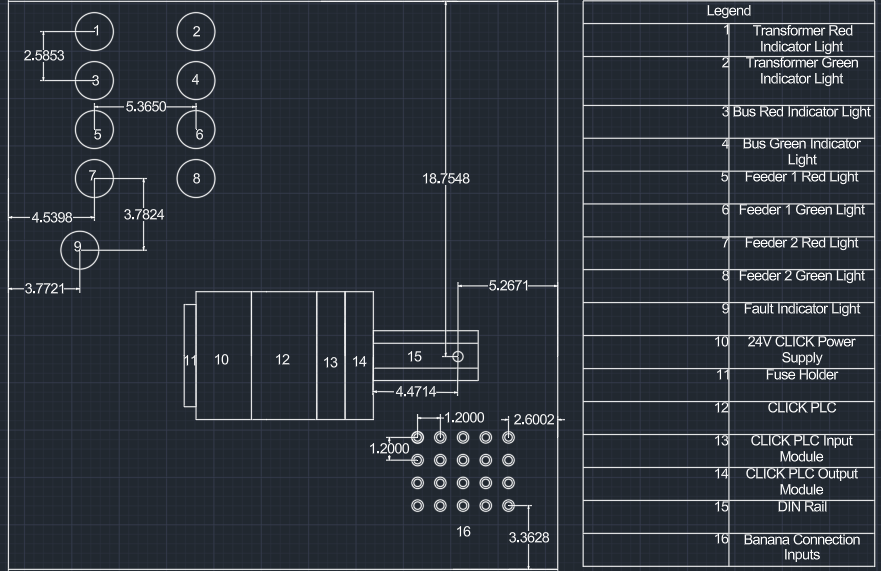
\includegraphics[width=0.95\textwidth]{Pictures/Subpanel_2.png}
	\end{center}
\end{figure}

\begin{figure}[H]
	\begin{center}
		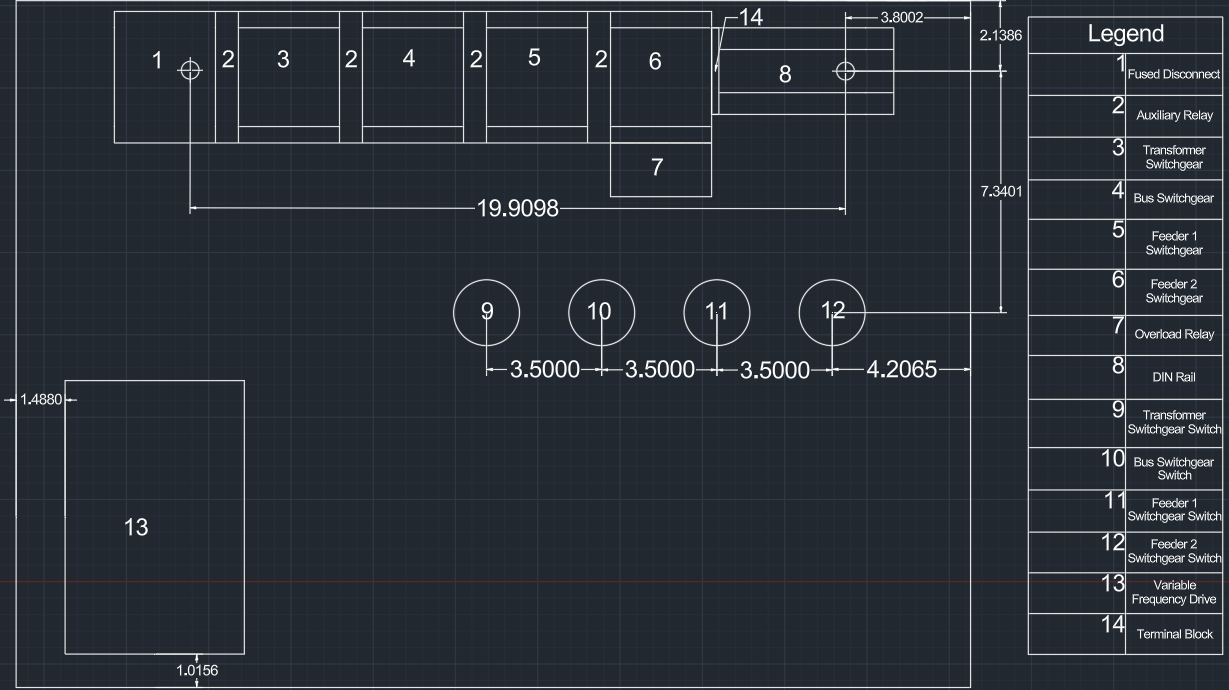
\includegraphics[width=0.90\textwidth]{Pictures/Subpanel_3.png}
	\end{center}
	\caption{Sub panel 2 diagram}\label{fig2:}
\end{figure}

\begin{figure}[H]
	\begin{center}
		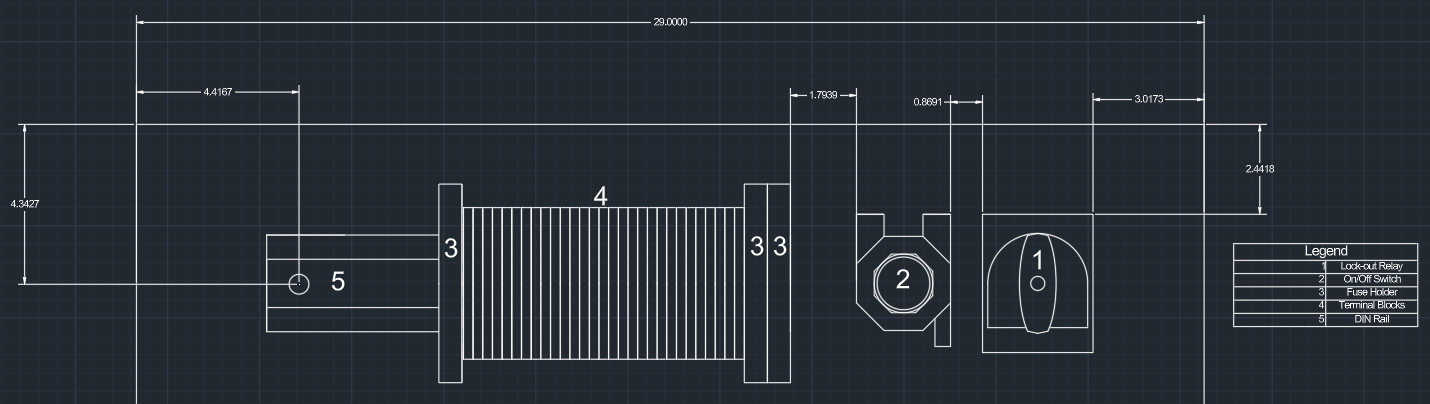
\includegraphics[width=0.95\textwidth]{Pictures/PLC_Subpanel_1.png}
	\end{center}
	\caption{Sub panel 1 diagram}\label{fig1:}
\end{figure}

\pagebreak

%----------------------------------------------------------------------------------------
%   Section: PLC ladder logic diagram
%----------------------------------------------------------------------------------------
\newpage
\section{PLC Ladder Logic Diagram}
\label{sec:plc}
\begin{figure}[H]
  \centering
  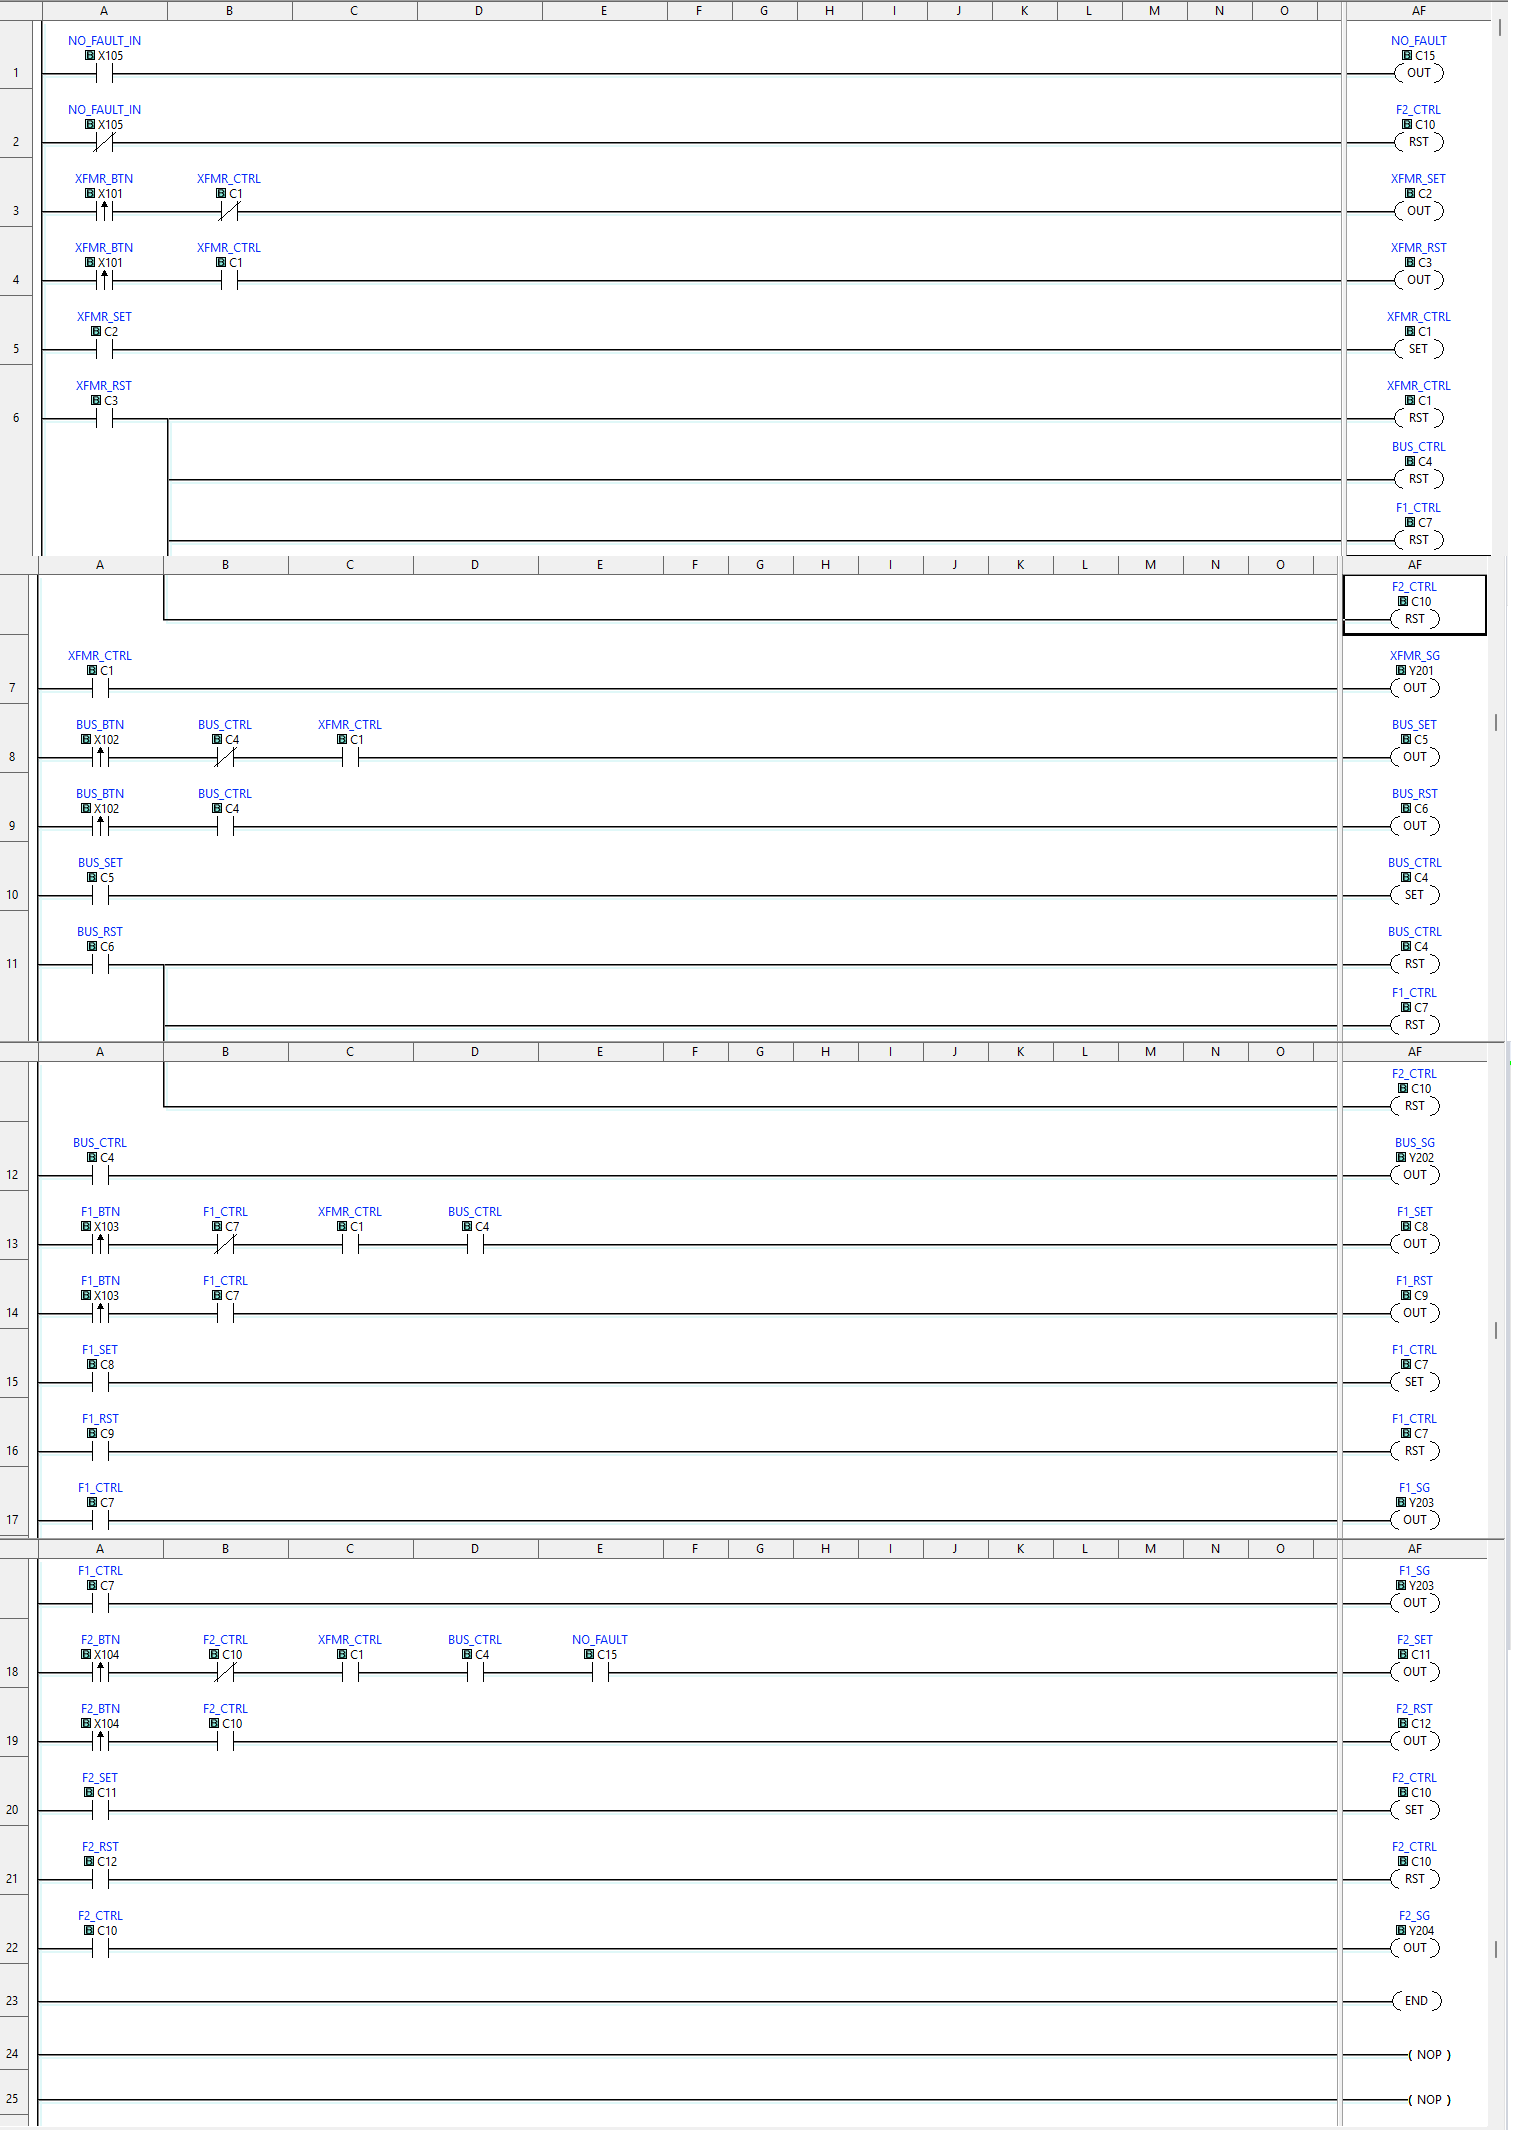
\includegraphics[width=.7\textwidth,keepaspectratio]{Pictures/LLD_CONSOL.png}
  \caption{PLC ladder logic using CLICK programming software}
\end{figure}

\pagebreak

%----------------------------------------------------------------------------------------
%   Section: Realized Specifications
%----------------------------------------------------------------------------------------
\newpage
\section{Realized Specifications}
\label{sec:specs}
\begin{enumerate}
	\item \emph{ The substation components shall be assembled according to the
		      one-line diagram shown in Figure 1.}\\
	      \textbf{The substation components are assembled according to the
		      one-line diagram shown in Figure 1.}

	\item \emph{ The substation electrical service shall be provided by a
		      variable three-phase 120/208 V source from the LabVolt 8821 power supply.}\\
	      \textbf{The substation electrical service is provided by a variable
		      three-phase 120/208 V source from the LabVolt 8821 power supply.}

	\item \emph{ The substation transformer shall be a
		      $\Delta$-$\Delta$ 208V/208V LabVolt 8348 three-phase transformer.}\\
	      \textbf{The substation transformer is a $\Delta$-$\Delta$ 208V/208V
		      LabVolt 8348 three-phase transformer.}

	\item \emph{ The load on feeder one shall be provided by a wye-connected
		      LabVolt 8311 resistive load bank and a delta-connected LabVolt 8331
		      capacitive load bank.}\\
	      \textbf{The load on feeder one is provided by a wye-connected
		      LabVolt 8311 resistive load bank and a delta-connected LabVolt 8331
		      capacitive load bank.}

	\item \emph{ The load on feeder two shall be provided by a LabVolt 8221
		      squirrel cage induction motor.}\\
	      \textbf{The load on feeder two is provided by a LabVolt 8221
		      squirrel cage induction motor.}

	\item \emph{ The mechanical load on the motor shall be provided by a
		      LabVolt 8960 Dynamometer.}\\
	      \textbf{The mechanical load on the motor is provided by a
		      LabVolt 8960 Dynamometer.}

	\item \emph{ Total load on both feeders shall not exceed the rated
		      capacity of the substation transformer.}\\
	      \textbf{The total load on both feeders is maintained below the rated
		      capacity of the substation transformer.}

	      % \item \emph{ Teams may develop a Python script that calculates loading
	      % 	      on the transformer for any combination of loading from the resistor
	      % 	      bank, cap bank, and motor.}\\
	      %       \textbf{A Python script was developed to calculate the loading on
	      % 	      the transformer for combinations of loading from the resistive
	      % 	      load bank, capacitive load bank, and induction motor.}
\end{enumerate}

\pagebreak

%----------------------------------------------------------------------------------------
%   Section: NFPA standards
%----------------------------------------------------------------------------------------
\newpage
\section{NFPA Standards}
\label{sec:nfpa_standards}
\paragraph{} For all NFPA 70 requirements the 2014 draft version was used.

\begin{itemize}
  \item Lockout/Tagout Procedure - Annex G {\newline} {\indent}
    We followed the sequence of the lockout/tagout procedure as relevant.
  \item Conductor sizing - 240.4(D)(1) - 310.15 {\newline} {\indent}
    18 gauge wire was used in the panel according with table 310.15(B)(16).
    This decision was based on an  expected expected maximum current
    draw of 0.982A for this control system.
    And is well under the maximum 7A that 18 gauge wire is allowed.
    % 0.9(power supply)+16m(PLC)+16m(inputs)+10m(outputs)+40m(both lights)=982mA
  \item Ampacity factor - 210.19(A)(1) - 210.20(A) {\newline} {\indent}
    Because this system will be operated as a continuous load the
    ampacity of the conductors used is not less
    than the noncontinuous load plus 125 percent of the continuous
    load. Making the minimum allowable ampacity
    1.22A, well within the 7A range.
    % 0.9(power supply)+16m(PLC)+16m(inputs)+10m(outputs)+40m(both lights)=982mA
  \item Fuse sizing - 240.6 {\newline} {\indent}
    Based on the max expected current draw of 0.982A and the NFPA
    paragraph listed we selected 1A fuses.
  \item Equipment grounding - 250.119 {\newline} {\indent}
    All grounding wires are green in compliance with the paragraph listed.
  \item Conductor location use - 310.10(A) {\newline} {\indent}
    All wires selected for this system are of type THHN. This wire is
    acceptable for the dry conditions in which
    our panel will operate.
\end{itemize}

\pagebreak

%----------------------------------------------------------------------------------------
%   Section: BOM
%----------------------------------------------------------------------------------------
\newpage
\section{Bill of Materials}
\label{sec:bom}
\begin{table}[!htp]\centering\small
	\caption{Bill of Materials}\label{tab: }
	\resizebox{\textwidth}{!}{
		\begin{tabular}{llrrrrrrr}\toprule
			               & Item                                                                             & Vendor            & Part Number       & Quantity & Price    & Extended Price \\\midrule
			               & \textbf{Rack Components}                                                         &                   &                   &          &          &                \\
			\textbf{1}     & Transformer Encap 500VA 277x240x208x120 to 240x120VAC                            & Automation Direct & C1FC50WE          & 1        & \$234.00 & \$234.00       \\
			\textbf{2}     & 12U Filler Panel with Stability Flanges (21")                                    & Rack Solutions    & 102-2142          & 2        & \$56.95  & \$113.90       \\
			\textbf{3}     & 3U Filler Panel with Stability Flanges (7")                                      & Rack Solutions    & 102-1824          & 1        & \$15.99  & \$15.99        \\
			\textbf{4}     & 4U Filler Panel with Stability Flanges (5")                                      & Rack Solutions    & 102-1825          & 1        & \$28.99  & \$28.99        \\
			\textbf{5}     & Rack 77" x 19", Al Finish                                                        & A-I Consolidated  & RR-1369-MG        & 1        & \$503.88 & \$503.88       \\
			\textbf{6}     & CLICK PLC                                                                        & Automation Direct & C0-11ARE-D        & 1        & \$247.00 & \$247.00       \\
			\textbf{7}     & CLICK power supply                                                               & Automation Direct & C0-01AC           & 1        & \$73.00  & \$73.00        \\
			\textbf{8}     & CLICK discrete input module, 8-point, 100-120 VAC                                & Automation Direct & C0-08NA           & 1        & \$63.00  & \$63.00        \\
			\textbf{9}     & CLICK discrete output module, 8-point, 17-240 VAC                                & Automation Direct & C0-08TA           & 1        & \$80.00  & \$80.00        \\
			\textbf{10}    & Casters, Hard Tread Composition, 2.75 in, 200 lbs, pair of 2                     & A-I Consolidated  & RC-7758-PR        & 2        & \$36.39  & \$72.78        \\
			\textbf{11}    & Safety Lockout Hasp                                                              & Grainger          & 1U177             & 1        & \$8.88   & \$8.88         \\
			\textbf{12}    & Push Button Safety Cover                                                         & Grainger          & 3PDE5             & 1        & \$120.09 & \$120.09       \\
			\textbf{13}    & Push Button                                                                      & Grainger          & 13Z546            & 1        & \$78.75  & \$78.75        \\
			\textbf{14}    & Lock Out Relay (Series 24)                                                       & Shallco           & 7601D             & 1        & \$224.00 & \$224.00       \\
			\textbf{15}    & Power Cord                                                                       & All Electronics   & LCAC-310          & 1        & \$6.00   & \$6.00         \\
			\textbf{}      &                                                                                  &                   &                   &          & .        &                \\
			\textbf{16}    & 3 phase power supply                                                             & LabVolt           & 8821              & 1        & \$196.00 & \$196.00       \\
			\textbf{17}    & 3 phase transformer                                                              & LabVolt           & 8348              & 1        & \$271.32 & \$271.32       \\
			\textbf{18}    & Resistive Load Bank                                                              & LabVolt           & 8311              & 1        & \$199.99 & \$199.99       \\
			\textbf{19}    & Capacitive Load Bank                                                             & LabVolt           & 8331              & 1        & \$199.99 & \$199.99       \\
			\textbf{20}    & Squirrel Cage Induction Motor                                                    & LabVolt           & 8221              & 1        & \$2,412.00 & \$225.00       \\
			\textbf{21}    & Dynanometer                                                                      & LabVolt           & 8960              & 1        & \$249.95 & \$249.95       \\
			\textbf{22}    & Fuse carrier, TeSys DF, 3P, 32A, 690VAC, fuse size 10x38mm, blown fuse indicator & Schneider         & DF103V            & 1        & \$56.32  & \$56.32        \\
			\textbf{23}    & Auxiliary contact block                                                          & Schneider         & LAD8N11           & 4        & \$24.59  & \$98.36        \\
			\textbf{24}    & 3 Phase Contactor                                                                & Schneider         & LC1D09            & 4        & \$62.40  & \$249.60       \\
			\textbf{25}    & Thermal overload relay, 1.2-1.8A adjustable, bi-metallic                         & Schneider         & LRD06             & 1        & \$40.95  & \$40.95        \\
			\textbf{26}    & Variable Frequency Drive                                                         & Automation Direct & GS13N-20P2        & 1        & \$164.00 & \$164.00       \\
			\textbf{27}    & DINnector screw single-level feedthrough terminal block, red                     & Automation Direct & DN-T12RED-A       & 8        & \$83.00  & \$664.00       \\
			\textbf{28}    & DINnector screw single-level feedthrough terminal block, green                   & Automation Direct & DN-T12GRN-A       & 3        & \$83.00  & \$249.00       \\
			\textbf{29}    & DINnector screw single-level feedthrough terminal block, white                   & Automation Direct & DN-T12W-A         & 12       & \$83.00  & \$996.00       \\
			\textbf{30}    & DINnector Terminal Block Fuse Holders                                            & Automation Direct & DN-F6FM           & 3        & \$168.00 & \$504.00       \\
			\textbf{31}    & USB to Ethernet Adapter                                                          & DigiKey           & U236-000-R        & 1        & \$26.31  & \$26.31        \\
			\textbf{32}    & Computer to CLICK PLC, ethernet cable                                            & Generic           & 887NC1            & 1        & \$12.35  & \$12.35        \\
			\textbf{33}    & CLICK Programming software                                                       & Automation Direct &                   &          & \$0.00   & \$0.00         \\
			\textbf{34}    & Pushbutton, Blue, IP65, 22mm, momentary, (1) N.O. contact(s)                     & Automation Direct & GCX1104           & 4        & \$9.00   & \$36.00        \\
			\textbf{35}    & Indicator Light, 22mm Non-Metal, 24VAC/DC Incan, Red                             & Schneider         & XB5AV64           & 4        & \$31.49  & \$125.96       \\
			\textbf{36}    & Indicator Light, 22mm Non-Metal, 24VAC/DC Incan, Green                           & Schneider         & XB5AV63           & 4        & \$31.49  & \$125.96       \\
			\textbf{37}    & Indicator Light, 22mm Non-Metal, 24VAC/DC Incan, Orange                          & Schneider         & XB5AV62           & 1        & \$31.49  & \$31.49        \\
			\textbf{38}    & Indicator Light, 22mm Non-Metal, 24VAC/DC Incan, Blue                            & Schneider         & XB5AVB6           & 1        & \$31.49  & \$31.49        \\
			\textbf{}      & \textbf{}                                                                        &                   &                   &          &          &                \\
			\textbf{}      & \textbf{Consumables}                                                             &                   &                   &          &          &                \\
			\textbf{39}    & Terminal Block Mounting Track, 17"                                               & Schneider         & 9080MH217         & 1        & \$3.68   & \$3.68         \\
			\textbf{40}    & Stranded Hook-up wire, 300V, UL1007, 18 AWG, red, 16/30 (100ft)                  & BulkWire.com      & Wire-ST-18-01-100 & 1        & \$21.44  & \$21.44        \\
			\textbf{41}    & Stranded Hook-up wire, 300V, UL1007, 18 AWG, green, 16/30 (100ft)                & BulkWire.com      & Wire-ST-18-01-101 & 1        & \$21.44  & \$21.44        \\
			\textbf{42}    & Stranded Hook-up wire, 300V, UL1007, 18 AWG, white, 16/30 (100ft)                & BulkWire.com      & Wire-ST-18-01-102 & 1        & \$21.44  & \$21.44        \\
			\textbf{43}    & Stranded Hook-up wire, 300V, UL1007, 18 AWG, blue, 16/30 (100ft)                 & BulkWire.com      & Wire-ST-18-01-103 & 1        & \$21.44  & \$21.44        \\
			\textbf{44}    & Stranded Hook-up wire, 300V, UL1007, 18 AWG, black, 16/30 (100ft)                & BulkWire.com      & Wire-ST-18-01-104 & 1        & \$21.44  & \$21.44        \\
			\textbf{45}    & Various 1 1/4" or 20 mm fuses                                                    & Mersen            & GGC1              & 3        & \$1.67   & \$5.01         \\
			\textbf{46}    & JUMPER 100/PK 3-POLE FOR MULTIPLE DINNECTOR TERM BLKS SCREWLESS                  & AutomationDirect  & DN-3J2Y           & 3        & \$72.00  & \$216.00       \\
			\textbf{Total} &                                                                                  &                   &                   &          &          & \$9,143.19     \\
			\bottomrule
		\end{tabular}
	}
\end{table}

\pagebreak

%----------------------------------------------------------------------------------------
%    APPENDICES
%----------------------------------------------------------------------------------------
% \newpage
% \appendix
%
% \section{Appendix: }
% \label{sec:App_}
% 

% \pagebreak

%----------------------------------------------------------------------------------------
%  BIBLIOGRAPHY
%----------------------------------------------------------------------------------------
% \newpage
% \bibliographystyle{unsrt}%Used BibTeX style is unsrt
% \bibliography{bibfile}
% \addcontentsline{toc}{section}{References}
%
%\nocite{MQTT_Py}

%----------------------------------------------------------------------------------------
%----------------------------------------------------------------------------------------
%    Section: Authors, Lab, Disclaimer & Acknowledgements
%----------------------------------------------------------------------------------------
% \newpage
% %\subsection*{PSU Power Engineering Laboratory}
%\noindent\small{Lab description...}

\subsection*{\textcolor{PSUgreen}{Authors}}
\noindent\textcolor{PSUblue}{\textbf{William Jeffreys}}\small{ } \\

\noindent\textcolor{PSUblue}{\textbf{Greyland Miller}}\small{ } \\

\noindent\textcolor{PSUblue}{\textbf{Rodney Downer}}\small{ } \\

\subsection*{\textcolor{PSUgreen}{Acknowledgements}}
\noindent{\small Funding for this research was provided by \dots.}

\subsection*{\textcolor{PSUgreen}{Disclaimer}}
\noindent{\small The contents of this report reflect the views of the authors, who are solely responsible for the facts and the accuracy of the material and information presented herein.  This document is disseminated under the sponsorship of COMPANY NAME in the interest of information exchange.}

% \pagebreak
%----------------------------------------------------------------------------------------

\end{document}
